%ltex: language=de-de
\chapter{Anhang A}
	\section{Pflichtenheft}
		\begin{table}[h]
			\centering
			\caption{Liste mit Festanforderungen.}
			\begin{tabular}{@{}p{.4\textwidth}p{.5\textwidth}@{}}
				\toprule
				\textbf{Festanforderungen} 						& \textbf{Erläuterung} \\
				\midrule
				Hygienisch										& Das Material muss Kontamination durch Verkeimung
				oder Ähnlichem weitestgehend unterbinden. Die Geometrie muss eine einfache und gründliche Reinigung ermöglichen.\\
				Thermisch geregelt								& Die Innentemperatur muss einstellbar sein und einem Regelkreis unterliegen.\\
				Thermische Isolierung							& Die innere Temperatur muss weitgehend stabil gehalten werden. \\
				Autarke Energieversorgung						& Erneuerbare Energien nutzend muss das Gerät über eine eigene Spannungsversorgung verfügen.\\
				Integrierter Energiespeicher					& Im Offline-Betrieb und bei Ausfall der eigenen Spannungsversorgung muss das Produkt betriebsfähig bleiben.\\
				\textit{Cradle-to-cradle}						& Sämtliche verbauten Komponenten müssen einem biologischen oder technischen Kreislauf zurückgeführt werden können.\\
				Kompakte und leichte Bauweise 					& Das Produkt muss beladen von einer Einzelperson transportiert werden können.\\
				Schockfreie Lagerung des Inhalts 				& Der Nutzraum muss von starken Erschütterungen entkoppelt sein.\\
				Alarmierung bei kritischer Temperatur			& Die Nutzenden müssen über kritische Temperaturzustände informiert werden.\\
				Alarmierung bei kritischem Akkustand			& Die Nutzenden müssen über kritische Energieversorgung informiert werden.\\
				\bottomrule
			\end{tabular}
		\end{table}
		% \newpage
		\begin{table}[h]
			\centering
			\caption{Liste nicht zu unter- oder gegebenenfalls überschreitender Parameter.}
			\begin{tabular}{@{}p{.4\textwidth}p{.5\textwidth}@{}}
				\toprule
				\textbf{Mindestanforderungen} 					& \textbf{Erläuterung} \\
				\midrule
				Kühlung \( \leq \SI{(-20 \pm 1)}{\celsius} \)	& Der Innenraum muss auf mindestens \SI{-20}{\celsius} heruntergekühlt werden können. \\
				Temperaturstabil \(\geq \SI{48}{\hour}\) 			& Die Temperatur muss min. \SI{48}{\hour} lang gehalten werden. \\
				Gewicht \(\leq \SI{20}{\kilo\gram}\)					& Die Box soll ein Leergewicht von max. \SI{20}{\kilo\gram} besitzen. \\
				\bottomrule
			\end{tabular}
		\end{table}
		% \newpage
		\begin{table}[h]
			\centering
			\caption{Liste von Eigenschaften, die das Produkt im Rahmen der Machbarkeit weiterhin aufweisen könnte.}
			\begin{tabular}{@{}p{.4\textwidth}p{.5\textwidth}@{}}
				\toprule
				\textbf{Wunschanforderungen} 											& \textbf{Erläuterung}\\
				\midrule
				Innenbeleuchtung 												& Bei schlechter Außenbeleuchtung sollte der Inhalt dennoch gut erkennbar sein.\\
				Statusanzeige													& Die Nutzenden sollen sich jederzeit über den Status des Produktes -- Temperatur,
				Leistungsaufnahme und -abgabe, Restkapazität -- informieren können.\\
				Modularer Aufbau												& Einzelne funktionale Komponenten sollen leicht austauschbar sein.\\
				Verbundbetrieb													& Mehrere der Produkte sollen im Verbund betrieben werden können. Hierzu zählt Stützbetrieb einzelner Geräte durch andere, sowie gesammelte Statusanzeige.\\
				Kompatibilität verschiedener ext. Spannungsversorgungen 		& Das Gerät soll an möglichst vielen verschiedenen externen Versorgungsspannungen betrieben werden können.\\
				\bottomrule
			\end{tabular}
		\end{table}

	\section{Marktforschung}
	Es wurden Marktforschungen betrieben, um eine Übersicht der konkurrierenden Kühlboxen zu erhalten.\par\medskip

	\textbf{T0022 FDN von} \href{https://www.eberspaecher-klima.de/fileadmin/data/corporatesite/pdf/de/4_air_conditioning/gp/fh_gp_kuehlcontainer_de.pdf}{\textsc{Eberspächer}}

	\begin{itemize}
		\item Temperatur von \SI{-24}{\celsius}
		\item Spannung \SI{12}{\volt} / \SI{24}{\volt} DC
		\item \SI{(65-70)}{\milli\metre} PU Wandausschämung
		\item Kältemittel R134a (Tetrafluorethan)
		\item Gewicht von \SI{20,5}{\kilo\gram}
		\item Außenabmessung 375 x 585 x 480 (BxTxH, Einheiten in mm)
	\end{itemize}

	\textbf{ICY 20 von} \href{https://www.frigolab.eu/gb/dometic-portable-freezers/67-icy-20.html#/47-normal_or_heated_refrigerator-heated_18c40c}{\textsc{FrigoLab Cold Technology}}

	\begin{itemize}
		\item Temperaturen von \SI{-18}{\celsius} bis \SI{10}{\celsius}.
		\item Außenabmessung 515 x 345 x 425 (BxTxH, Einheiten in mm).
		\item Digitales Display.
		\item Kühlung durch einen Kompressor.
		\item Kältemittel R134a (Tetrafluorethan).
		\item Versorgung von \SI{12}{\volt} / \SI{24}{\volt} DC oder \SI{230}{\volt} AC.
		\item Gewicht von \SI{18}{\kilo\gram}.
		\item Resistent gegen Schock und mechanische Belastungen.
		\item CFC- und HCF-freie Polyurethanschaum.
	\end{itemize}

	\textbf{TC 702 von} \href{https://www.tritec-klima.de/datenblaetter/de/kaelte/portable/TD-TC702.pdf}{\textsc{Tritec}}

	\begin{itemize}
		\item Temperaturen von \SI{-24}{\celsius} bis \SI{10}{\celsius}.
		\item Außenabmessung 375 x 585 x 480 (B x T x H, Einheiten in mm).
		\item Durch Autobatterie mit \SI{12}{\volt} / \SI{24}{\volt} DC betrieben.
		\item Umschalter für Netzbetrieb (\SI{230}{\volt} AC).
		\item Stabiler und stoßfester UVA-beständiger Kunststoff.
		\item Deckel mit spezieller Verriegelung.
		\item Dämmung mit FCKW-feiem PU-Hartschaum von \SI{80}{\milli\metre} Dicke.
		\item Reinigungsmittelresistent.
		\item Alarmmeldungen bei möglichen Fehlern des Gerätes.
		\item Kompressor mit einem R52A Kältemittelgemisch.
	\end{itemize}

	\textbf{T0022/T0032 von} \href{https://coldtainerusa.com/wp-content/uploads/2020/03/Product_Info_T0022-T0032_US_ColdtainerUSA-1.pdf}{\textsc{Coldtainer}}

	\begin{itemize}
		\item Temperatur von \SI{-24}{\celsius} bis \SI{40}{\celsius}
		\item Spannungsversorgung 12 / \SI{24}{\volt} DC %volt of direct current bzw. Gleichstrom
		\item \SI{(65-70)}{\milli\metre} PU-Wandausschämung
		\item Kältemittel R134a (Tetrafluorethan)
		\item Gewicht von \SI{20,5}{\kilo\gram}
		\item \(\approx \SI{23}{L}\) Kapazität
	\end{itemize}

	\section{Mindmap}
	Nach den ersten Überlegungen zu den Anforderungen und Funktionen des Transportgefäßes kann eine Übersicht anhand eines Mindmaps wie in Abb. \ref{fig:mindmap} gestaltet werden.
	\begin{figure}[H]
		\centering
		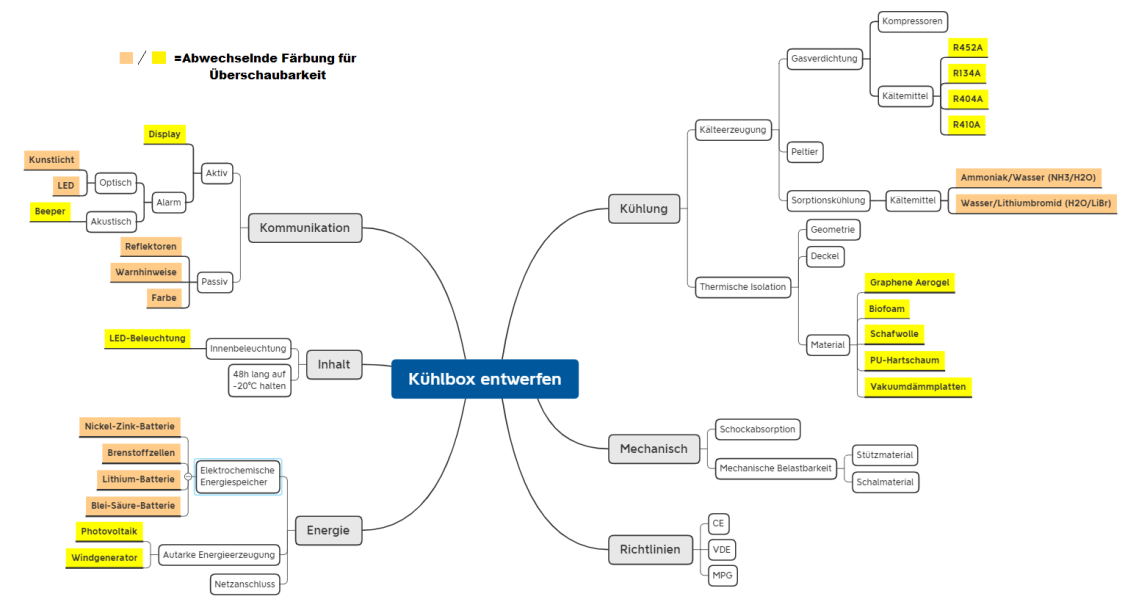
\includegraphics[angle=90,width=0.8\linewidth]{assets/skizzen/Mindmap}
		\caption{Mindmap.}
		\label{fig:mindmap}
	\end{figure}

	\section{Materialien und Regularien}
		\subsection{Normen und Regularien}
			Dem \textsc{Bundesinstitut für Arzneimittel und Medizinprodukte} zu Folge ist \enquote{ein Absehen von der Genehmigung einer klinischen Prüfung} \cite{genehmigungspflicht.BfArM}
			möglich, wenn das Produkt etwa den Medizinprodukten der Klasse I zuzuordnen ist \cite{MPG}. Die Klassifizierung von medizinischen
			Produkten wiederum ist durch die \textit{Richtlinie 93/42/EWG} geregelt. In \textit{Anhang IX} ist zu lesen:
			\begin{quote}
				\enquote{Alle nicht invasiven Produkte gehören zur Klasse I [..]} \cite{directive.93-2-EC.medizinprodukte.2007}
			\end{quote}
			mit Ausnahme derer nicht-invasiven Produkte, die in folgenden Punkten aufgeführten Regelungen Anwendung finden.
			Es ist anzunehmen, dass dies hier \underline{nicht} der Fall ist.\par\medskip

			Dennoch handelt es sich um ein Gerät, dass, um für den europäischen Markt zugelassen werden zu können eine \underline{CE-Kennzeichnung}
			benötigt und somit die damit verbundenen Auflagen erfüllen muss. Die relevante Norm scheint hier \textsc{DIN EN 60601}.\par
			Weiter wird eine \underline{VDE-Kennzeichnung} benötigt, da es sich um ein in einer Form elektrisch betriebenes Gerät handelt.
			Dies wird um so relevanter, wenn ein Betrieb an Netzspannung möglich oder vorgesehen ist.

		\subsection{Auswahl Dämmmaterialien}
			\begin{table}[H]
				\centering
				\caption{Übersicht möglicher Materialien zur thermischen Dämmung.}
				\begin{tabular}{@{}lrrrr@{}}
					\toprule
					(Handels-)Name																& \(\lambda / \frac{mW}{m \cdot K}\)	& \(\rho / \frac{mg}{cm^3}\)	& E-Modul / \(kPa\) 				& Druckfestigk. / \(kPa\) \\
					\midrule
					Luft 																		&\(25,7\)						&\(1,2041\)						&--									&-- \\
					&&&&\\
					Graphen/Silizium Aerogel \cite{silica.graphene.aerogel.Lei.2017} 			& \(7,3\) -- \(9\)			&								&\((2,4\) -- \(4\))\(\cdot 10^3\)	&\\
					Biofoam (Algen) \cite{Biofoam2.Morrison.1994}								&								&30								&									&\\
					Biobasiertes PU \cite{Biobased.PU.HuangX.QiJ.DeHoopC.XieJ.andChenY.2017}	&\(33\)							&\(18,5\)						&\(176,7\)							&\(15,4\)\\
					Air laid feather fibre \cite{air.laid.feather.fibre.Zhao.2020} 				& \(30^1\)		&								&									& \( > 30^2 \) \\
					&&&&\\
					Vakuumdämmplatte \cite{Vakuumplate.Nagarajan.2013}							&\(37\) -- \(31\)			&\(16,3\) -- \(59,4\)		&									&\\
					\bottomrule
				\end{tabular}
				\label{tab:isomaterial}
			\end{table}
			\( ^1 \)Bei \SI{-10}{\celsius}\\
			\( ^2 \)Nach 10 minütigem Eintauchen in flüssigen Stickstoff (\SI{-195}{\celsius})

	\section{Überschlagsrechnung Energiebedarf}
		\textit{Annahme}:
		\SI{20}{\litre} Innenraum; zu \SI{80}{\percent} gefüllt mit Wasser (\( \SI{16}{\litre} \widehat{=} \SI{16}{\kilo\gram} \))\par\medskip
		\textit{Betrachtung:}
		Energien beim Herunterkühlen von Wasser bei RT (\( \SI{20}{\celsius} = \SI{293}{\kelvin} \)) auf \( \SI{-20}{\celsius} = \SI{253}{\kelvin} \)\par\bigskip
		\par\bigskip
		\underline{Je kg umgewandelte Wärmeenergie \(=\) Änderung der spezifischen Enthalpie:}\par\medskip
		Für \SI{20}{\celsius} \(\rightarrow\) \SI{0}{\celsius}:
		\begin{align}
			\Delta h_1	&= \frac{\Delta Q_1}{m} = c_{Wasser} \cdot \left(T_0 - T_{20}\right) = \SI{4,19}{\kilo\joule\per\kilo\gram\kelvin}\\% \cdot \left(\SI{273}{\kelvin} - \SI{293}{\kelvin}\right) \nonumber\\
						&= \SI{-83}{\kilo\joule\per\kilo\gram}
		\end{align}
		Zum Erstarren:
		\begin{align}
			\Delta h_2	&= h_{erstarr,Wasser} = -h_{fus,Wasser} \nonumber \\
						&= \SI{-334}{\kilo\joule\per\kilo\gram}
		\end{align}
		Für \SI{0}{\celsius} \(\rightarrow\) \SI{-20}{\celsius}:
		\begin{align}
			\Delta h_3	&= c_{Eis} \cdot (T_{-20}-T_0) = \SI{2,0}{\kilo\joule\per\kilo\gram\kelvin} \cdot (\SI{253}{\kelvin}-\SI{273}{\kelvin}) \nonumber \\
						&= \SI{-40}{\kilo\joule\per\kilo\gram}
		\end{align}

		\begin{align}
			\Delta h_{ges} 				&= \Delta h_1 + \Delta h_2 + \Delta h3 = \SI{-83,8}{\kilo\joule\per\kilo\gram} - \SI{334}{\kilo\joule\per\kilo\gram} - \SI{40}{\kilo\joule\per\kilo\gram} = \underline{\SI{-457,8}{\kilo\joule\per\kilo\gram}} \nonumber \\
			\Rightarrow \Delta Q{ges} 	&= \Delta h_{ges} \cdot m = \SI{-457,8}{\kilo\joule\per\kilo\gram} \cdot \SI{16}{\kilo\gram} \nonumber \\
										&= \SI{-7324,8}{\kilo\joule} \approx \underline{\underline{\SI{-7,3}{\mega\joule}}}
		\end{align}

		\underline{Benötigte Energie, um eine Temperaturdifferenz aufrechtzuerhalten:}\par\smallskip
		Mit einer Schichtdicke des thermischen Isoliermaterials von \(l = \SI{0,05}{\metre}\), der Gesamtfläche \(A\) des Kühlraums von \(\approx \SI{0,208}{\metre\squared}\)
		und einer thermischen Leitfähigkeit von \(\lambda = \SI{7,3}{\mW\per\metre\kelvin}\) lässt sich der thermische Widerstand zu
		\(R_{th} \approx \SI{33}{\kelvin\per\watt}\) abschätzen.
		\begin{equation}
			R_{th} 	= \frac{l}{\lambda \cdot A} = \frac{\SI{0,05}{\metre}}{\SI{7,3}{\mW\per\metre\kelvin} \cdot \SI{0,208}{\metre\squared}} \approx \SI{33}{\kelvin\per\watt}
		\end{equation}

		\begin{align}
			\dot{Q} = P	&= \frac{(T_{aussen} - T_{innen})}{R_{th}} \nonumber\\
						&= \frac{\SI{313,15}{\kelvin} - \SI{253,15}{\kelvin}}{\SI{33}{\kelvin\per\watt}} \nonumber\\
						&\approx \SI{1,81}{\watt} \\
			\Rightarrow &\approx \SI{87,27}{\watt\hour} \qquad \text{(Für \SI{48}{\hour})} \nonumber
		\end{align}
		%
		Bei einer Außentemperatur von \SI{40}{\celsius} und einer Anfangsinnentemperatur von \SI{-20}{\celsius} mit der Annahme, dass \SI{33}{\percent} des Nutzvolumens von \SI{16,72}{\litre} mit Wasser und
		\SI{66}{\percent} mit Luft gefüllt sind, wird von einer Dauer von \(t_{krit} = \SI{14,2}{\hour}\) ausgegangen, bis sich der Innenraum um \SI{2}{\kelvin} erwärmt hat.
		\begin{align}
			t_{krit}	&= \frac{\Delta T}{\dot{Q}} \cdot \left[\left(0,66 \cdot \rho_{aq}V \cdot c_{aq}\right) + \left(0,33 \cdot \rho_{luft}V \cdot c_{luft} \right)\right] \nonumber \\
						&= \frac{\SI{2}{\kelvin}}{\SI{1,81}{\watt}} \cdot \bigg[\left( 0,66 \cdot \SI{1000}{\kilo\gram\per\metre\cubed} \cdot \SI{0,0167}{\metre\cubed} \cdot \SI{4200}{\joule\per\kilo\gram\kelvin}\right)\nonumber \\
						&+ \left(  0,33 \cdot \SI{1,225}{\kilo\gram\per\metre\cubed} \cdot \SI{0,0167}{\metre\cubed} \cdot \SI{1005}{\joule\per\kilo\gram\kelvin} \right)\bigg] \nonumber \\
						&\approx \SI{51.159}{s} \approx \SI{14,2}{h}
		\end{align}
		\begin{align}
			\Delta T	&= \frac{\Delta Q}{0,66 \cdot \rho_{aq}V \cdot c_{aq}}\nonumber\\
								&= \frac{\SI{1,81}{\watt} \cdot \SI{5}{\hour} \cdot \SI{3600}{\second \per \hour} }{0,66 \cdot \SI{997}{\kilogram \per \metre\cubed} \cdot \SI{ (16,72 \cdot 10^{-3}) }{ \metre\cubed } \cdot \SI{4200}{\joule \per \kilogram \kelvin}}\nonumber\\
								&\approx \SI{0,7}{\kelvin}
		\end{align}

		%=============== ???REDUNDANT??? ==================
	% \section{Realisierung}
	% 	\begin{align*}
	% 		\dot{Q} = P &= \frac{\lambda \cdot A \cdot (T_{aussen} - T_{innen})}{d} \\
	% 					&= \frac{\SI{0,009}{\watt\per\metre\kelvin} \cdot \SI{431857,65 \cdot 10^{-6}}{\metre\squared} \cdot (\SI{313,15}{\kelvin} - \SI{253,15}{\kelvin})}{\SI{50 \cdot 10^{-3}}{\metre}} \\
	% 					&\approx \SI{4,66}{\watt} \\
	% 		\Rightarrow &\approx \SI{223,88}{\watt\hour} \qquad \text{(Für \SI{48}{\hour})}
	% 	\end{align*}
	% 	%
	% 	\begin{align*}
	% 		\Delta T 	&= \frac{\Delta Q}{m \cdot c_{H_2O,liq}} \\
	% 					&= \frac{\SI{4,66}{\watt} \cdot \SI{5}{h}}{\SI{10}{\kilo\gram} \cdot \SI{4,2 \cdot 10^{3}}{\joule\per\kilo\gram\kelvin}} \cdot \SI{3600}{\second\per\hour} \\
	% 					&\approx \SI{2}{\kelvin}
	% 	\end{align*}
	%=================================================
	
	\section{Dimensionierung Photovoltaikmodul}
	Mithilfe der Photovoltaik kann der Akku bei Tageslicht geladen und die Kühlung somit aufrecht erhalten werden. Hierbei ist einem monokristallines PV-Modul bei einer Fläche
	von $ \SI{9}{m^2} $ eine Spitzenleistung von mindestens $ \SI{1}{kW_p} $ zu entnehmen \cite{Wesselak.photovoltaik.2012}. Zum Betrieb des \textit{nICE.cube} und Laden seines Energiespeichers ist ein
	Viertel der Leistung ($ \widehat{=} \SI{250}{W_p} $) ausreichend. Dies entspricht einer effektiven Fläche von $ \SI{2,25}{m^2} $
		
	\section{Volumenberechnung}
		Das Nutzvolumen setzt sich aus der Länge $ L $, Breite $ B $ und Höhe $ H $ der inneren Box zusammen.
		
		\begin{align}
		V_{nutz} &= L \cdot B \cdot H \nonumber \\
		&= \SI{4,00}{dm} \cdot \SI{2,48}{dm} \cdot \SI{1,73}{dm} \nonumber \\
		&= \SI{17,16}{L}
		\end{align}
		
		Im Sinne thermischer und mechanischer Optimierung wurden Verrundungen mit \(r=\SI{4}{\mm}\) entlang der Innenkanten des Nutzvolumens platziert. Diese reduzieren das
		effektive Nutzvolumen auf $ \SI{16,72}{L} $.
		
	\section{Elektronik}
		Die Verbindung der jeweiligen Elektronikkomponenten wird in \cref{fig:schaltschema} schematisch dargestellt.
		
		\begin{figure}[H]
			\centering
			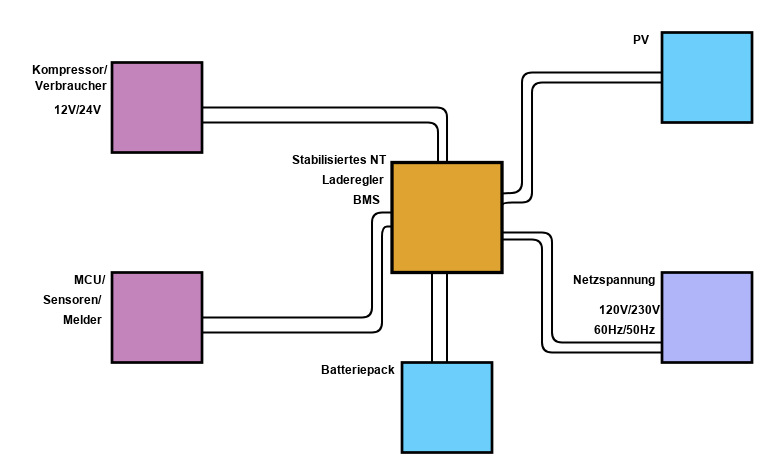
\includegraphics[width=1\linewidth]{assets/skizzen/Schaltschema}
			\caption{Schaltschema der Elektronik.}
			\label{fig:schaltschema}
		\end{figure}

		Sowohl die interne als auch sämtliche externe Spannungsversorgungen werden vom internen Netzteil auf den Lastkreis von \SI{12}{V}, sowie die Versorgungsspannung der Boardelektronik
		geregelt. Das im Netzteil integrierte Batteriemanagement übernimmt hierbei die Überwachung des Akkuzustandes. Daten wie Außen- und Innentemperatur, Temperatur der Akkuzellen,
		Statistiken zum Zustand des Akkus etc. laufen zentral im Mikrocontroller zusammen, werden dort verarbeitet und gegebenenfalls an die Meldesysteme weitergegeben.

		Um Raum einzusparen und das Kühlkonzept der Boardelektronik zu vereinfachen wurden in der Realisierung Mikrocontroller, Batteriemanagement und Netzteil in einem Bauteil vereint
		(Pos. 8 in \cref{tab:stueckliste}).